\documentclass[11pt,letterpaper]{article}

\usepackage[letterpaper,margin=0.8in,nohead]{geometry}

\usepackage[colorlinks]{hyperref}
\usepackage{url}
\usepackage{breakurl}
\usepackage[T1]{fontenc}

\hypersetup{
	colorlinks,
	linkcolor={red},
	citecolor={red},
	urlcolor={blue}
}

\usepackage{verbatim}
\usepackage{fancyvrb} 
\usepackage{scrextend}
\usepackage{enumitem}
\usepackage{url}
\usepackage{tabularx}

\usepackage{caption}
\usepackage{graphicx}
\usepackage{subcaption}

\usepackage{changepage}   % for the adjustwidth environment

\newenvironment{answer}{\em \color{blue} \begin{adjustwidth}{1cm}{1cm}}{\end{adjustwidth}}

% math
\usepackage{amsthm,amsmath}
\usepackage{amsfonts}

\newcommand{\mc}[1]{\mathcal{#1}}	% Mechanisms / Algorithms
\newcommand{\rv}[1]{\mathbf{#1}}    % Random variable

\newcommand{\pr}[1]{\mathrm{Pr}\{#1\}} % Probability

\newtheorem{corollary}{\bf Corollary}%[theorem]
\newtheorem{lemma}{\bf Lemma}%[theorem]
\newtheorem{definition}{\bf Definition}%[section]

\newtheorem{observation}{\bf Observation}%[theorem]

% load cleveref last!
\usepackage[capitalise]{cleveref}


\begin{document}
	
	\title{EN4720: Security in Cyber-Physical Systems \\ Exercise --- Application Security}
	
	%% This is an individual assignment!!
	%% TODO: put your name and index number here here!
	\author{ \textcolor{blue}{Name: Thalagala B. P.} \\ \textcolor{blue}{Index No: 180631J}}
	
	\maketitle
	
	\begin{center}
		\color{red}\bf This is an individual exercise! \\ Due Date: 20 June 2023 by 11.59 PM
	\end{center}
	
	\vspace{1in}
	
	This exercise has to be carried out using a \textcolor{red}{Linux-based virtual machine}. Read all the instructions and questions before attempting the exercise. Add answers under each question in the Questions section and submit the resulting PDF.
	
	\subsection*{Instructions}
	
	\begin{enumerate}
		\item Objective of this exercise is to perform a web application security assessment using OWASP ZAP (Zed Attack Proxy) on Ubuntu and identify potential vulnerabilities based on the OWASP Top 10 (2017) list. Download and install the latest version of OWASP ZAP from the official OWASP ZAP website (\href{https://www.zaproxy.org/download/}{https://www.zaproxy.org/download/}).
		
		\item Make sure you are using a virtual machine (such as VirtualBox or VMware), which is set to NAT networking mode.
		
		\item Download and install DVWA (Damn Vulnerable Web Application) on your Ubuntu system. You can find the installation instructions and the necessary files on the official \href{https://github.com/digininja/DVWA}{DVWA GitHub repository}. Please follow the steps carefully in the GitHub repository.
		
		\item Configure Proxy Settings: Configure your web browser or system network settings to use OWASP ZAP as a proxy. This will allow OWASP ZAP to intercept and analyze the web application's traffic.
		
		\item Scan for Vulnerabilities: Use OWASP ZAP to perform an active, automated scan on the DVWA application. OWASP ZAP will analyze the captured traffic and identify potential vulnerabilities within DVWA. You will have to analyze the results and detect which OWASP Top 10 category each vulnerability belongs to.
		
	\end{enumerate}
	
	\newpage
	\subsection*{Questions}
	
	For all the questions in this section, add a screenshot of the terminal (including all the commands you ran to perform the task) unless specified otherwise. The evaluator should be able to see each step that you followed to perform each task. In all screenshots, the areas marked (which are unique to your terminal display) in Figure 1 (the sample answer to Question 1) must be visible.
	
	\begin{enumerate}
		
		\item View the currently logged in user.
		
		\begin{figure}[h]
			\centering
			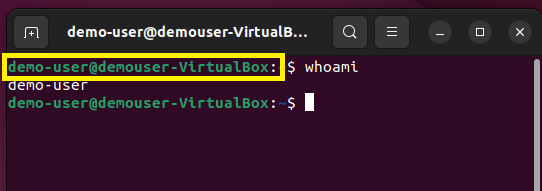
\includegraphics[width=0.65\columnwidth]{images/ex4-sample-terminal-output.png}
			\caption{Sample Terminal Output} \label{fig:sample-terminal-output}
		\end{figure}
		
		\item Using the  \textbf{ifconfig} command, check your network settings and determine if your network is configured to use NAT (Network Address Translation). Provide a screenshot of the ifconfig output and explain how to identify the use of NAT by examining the network information displayed in the  \textbf{ifconfig} output.
		
		\begin{answer}
			%% TODO: Add answer here
			Your answer here
		\end{answer}
		
		
		
		\item Follow the instructions in github repository and add a screentshot of the database credentials. You may use vim command to check default credentials in \textbf{./config/config.inc.php} file.
		
		\begin{answer}
			%% TODO: Add answer here
			Your answer here
		\end{answer}
		
		\item Add a screenshot of the list of detected vulnerabilities.
		
		\begin{answer}
			%% TODO: Add answer here
			Your answer here
		\end{answer}
		
		\item Briefly describe each detected vulnerability.
		
		\begin{answer}
			%% TODO: Add answer here
			Your answer here
		\end{answer}
		
		\item Complete the below table by identifying each vulnerability, including its impact, detected source paths, evidence, and potential OWASP top 10 attack scenarios.
		
		\begin{answer}
			\begin{table}[h!]
				\caption{Vulnerability details} \label{tab:Vulnerability details}
				\begin{tabularx}{\columnwidth}{|p{3.7cm}|p{1.5cm}|X|p{4.2cm}|}
					\hline
					\textbf{Vulnerability} &  \textbf{Impact} & \textbf{Evidence} & \textbf{Potential OWASP top 10 attack scenarios}\\
					\hline
					Absence of Anti-CSRF Tokens & Medium & <form action="\#" method="post"> & CSRF\\\hline
				\end{tabularx}
			\end{table}
		\end{answer}
		
		\item Identify solutions for each listed vulnerability.
		
		\begin{answer}
			%% TODO: Add answer here
			Your answer here
		\end{answer}
		
	\end{enumerate}
	
\end{document}